\subsection{Design three}
\label{design3}
\subsubsection*{Description}
The idea behind this design is to come as close to preexisting methods of controlling a vehicle game without the need for buying a controller. This should be done by only utilizing a single standard webcam and color recognition for tracking controls and functionalities. The user is required to make/or obtain any desired material that the user wishes to use as controller material e.g. cardboard, piece of paper, etc. (theoretically any object should be viable). Thereafter create the desired shape and size representing the steering wheel. 
Additionally, BLOBs (See section \ref{sec:blob}) will be used to control the game. 
\begin{figure}[h]
\centering
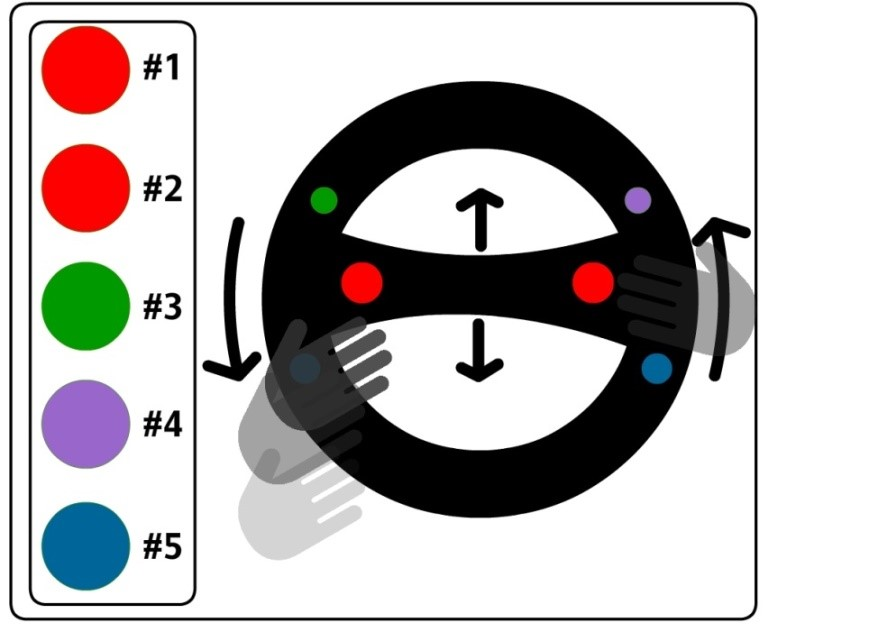
\includegraphics[scale=1]{Design31}
\caption{Controller: Blob and movement description}
\label{fig:design31}
\end{figure}

As seen on figure \ref{fig:design31}, BLOB \#1 \& \#2 is for implementing rotation and depth for controlling the vehicle forward, backward, and breaking. These BLOBs must be visible and placed adjacent and horizontal to one another. This is to ensure that the tracking of rotation and depth is possible.

Additionally, the BLOBs \#3, \#4 and \#5 will be visible, but perform no functionality before the user blocks the BLOB and thereby activating the desired function/ability of the designated BLOB. By utilizing this method, the procedure of pressing a button is reconstructed and therefore imitates a real controller.
\bigskip

\subsubsection*{Functionality description} \label{Dfunc}

\begin{figure}[h]
\centering
\caption{BLOB blocking illustration}
\label{fig:design32}
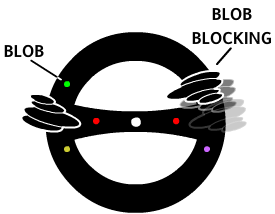
\includegraphics[scale=.75]{Design32}
\end{figure}

\begin{figure}[h]
\centering
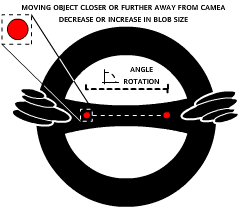
\includegraphics[scale=.75]{Design33}
\caption{Rotation \& forward/Backward}
\label{fig:design33}
\end{figure}

By implementing functionalities that is activated by blocking specific BLOBs, it is possible to add numerous functionalities by just adding more BLOBs to the controller. 

By designing the controls in this specific manner, the activation would, theoretically, be easily accessible. This will make it possible for the user to quickly activate certain functionalities or make a specific row of operations, which with movement could be somewhat problematic to perform simultaneously. 

One negative aspect of the technique is that it is likely that depending on the positioning of the BLOBs, several functionalities might be accidentally activated. Furthermore, since the controller will have to be positioned towards the webcam in order to track the BLOBs, the user will not be able to see the designated “button” that is present on the controller, and will therefore have to remember the placement of them and will only get feedback from the performed action, in game, if the action is registered in the first place.


\subsubsection*{Compared to the List Of Requirements and Final Problem Statement.}
As described in the Final Problem Statement (Section: \ref{sec:fps}, page \pageref{sec:fps}), the following functionalities are implemented:

\begin{itemize}
\item Steering left and right (See fig. \ref{fig:design31})
	\begin{itemize}
	\item Two BLOBs placed horizontally adjacent to each other will make it possible to detect rotation and therefore making it possible to steer a vehicle.
	\end{itemize}
	
\item Moving forward \& backward/breaking (See fig. \ref{fig:design33})
	\begin{itemize}
	\item By moving the object closer or further away, the program is able to detect the movement and therefore simulate the vehicle moving forward, backward or braking.
	\end{itemize}
	
\item Shift gears
	\begin{itemize}
	\item By implementing two BLOBs with separate colors, when the specific BLOB is blocked and therefore not visible, the implemented functionality of gear shift is activated, up or down depending on the implemented functions.
	\end{itemize}
	
\item Utility Button(s)
	\begin{itemize}
	\item For each game, there are several functionalities which are specific for that game. Therefore a BLOB, with the same procedure as the BLOBs for shifting gears will be implemented.  That will have functionalities which will be defined by the specific vehicle game that is being played. This can be extra utilities such as power boost, attack, etc.
	\end{itemize}
\end{itemize}

\subsubsection*{Pros and cons}
Pros:
\begin{itemize}
\item The user is able to create a controller with a shape and size, which is suitable for the individual’s preferences.
\item The required BLOBs except the two red BLOBs that is used for rotation and depth, can be placed anywhere on the assembled controller which is suitable for the individual preferences of the player. 
\item Since activation of functionalities only requires that a certain BLOB is blocked, possibly several functions can be activated simultaneously or rapidly after one another without much delay or effort based on the positioning of the BLOBs.
\item It is possible to implement a large number of additional functionalities.
\end{itemize}
Cons:
\begin{itemize}
\item As mentioned in Functionality description (\ref{Dfunc}); By implementing several features and functionalities it is possible to cover several BLOBs by accident and therefore activate undesired functionalities.
\end{itemize}
